\documentclass[oneside,mtp]{iiitg}
\let\mydegree\degree
\let\degree\relax
%
% The rest of the class options are the same as the regular book class.
% A few to remember:
%
%   oneside : Produces single sided print layout (recommended for theses less than 50 pages)
%   twoside : Produces single sided print layout (the default if you remove oneside)
%
% The BYUPhys class provides the following macros:
%
%   \makepreliminarypages : Makes the preliminary pages
%   \clearemptydoublepage : same as \cleardoublepage but doesn't put page numbers
%                           on blank intervening pages
%   \singlespace          : switch to single spaced lines
%   \doublespace          : switch to double spaced lines
%
% --------------------------- Load Packages ---------------------------------

% The graphicx package allows the inclusion of figures.  Plain LaTeX and
% pdfLaTeX handle graphics differently. The following code checks which one
% you are compiling with, and switches the graphicx package options accordingly.



\usepackage{makecell,tabularx} % for 'tabularx' env. and 'X' col. type
%\renewcommand\theadfont{\normalsize}
\usepackage{longtable}
%usepackage[shortlabels]{enumitem}
%usepackage{setspace}
\usepackage{emptypage}
\usepackage{changepage,ifthen}
%\textwidth 6.5in
%\addtolength{\oddsidemargin}{-.5in}
%\textheight 10in
%\addtolength{\topmargin}{-1in}
\addtocounter{secnumdepth}{2}
%\setlength{\parindent}{0pt}
\usepackage{algorithm}
\usepackage{algorithmic}
\usepackage{hyperref}
\usepackage{graphicx}
\usepackage{pdfpages}
\usepackage{epsfig}
\usepackage{amsmath}
%\usepackage{geometry}
%\usepackage{setspace}
%\usepackage{arydshln}
\usepackage{amsmath,amssymb,verbatim,eufrak}
\usepackage[dvips,colorlinks,bookmarksopen,bookmarksnumbered,citecolor=red,urlcolor=red]{hyperref}

%\usepackage{natbib,stfloats}
\usepackage{mathrsfs}
%\usepackage{algorithm}
\usepackage{algpseudocode}
\usepackage{xltabular}
%\usepackage{fixltx2e}
%\usepackage{stfloats}

\usepackage{float}
\usepackage[hyphens]{url}
\urlstyle{rm}
%\usepackage{breakurl}
%\usepackage{hyperref}
%\def\UrlBreaks{\do\/\do-}
\usepackage{arydshln}
\algtext*{EndIf}

%\usepackage{babel}
%\usepackage{enumitem}
\newcommand{\kthead}[1]{\multicolumn{1}{c}{\bfseries #1}}
%koeradoera added above 3 lines
\usepackage{program}
%above line koeradoera added

\usepackage{comment}
%above line added by koeradoera
\usepackage{amsfonts}
%\usepackage{amssymb}
%\usepackage[centertags]{amsmath}
\usepackage{epsfig}
\usepackage{epstopdf}
\usepackage{enumerate}
\usepackage{graphicx}
\usepackage{graphics}
\usepackage{subfig}
\usepackage{multirow}
\usepackage{rotating}
\usepackage{times}
\usepackage{lscape}
\usepackage[bottom]{footmisc}
\usepackage{booktabs}
\usepackage{colortbl}
\usepackage{threeparttable}
%\usepackage{algorithm}

\usepackage{algorithmicx}

%\usepackage[lined,algonl,algochapter,algoruled]{algorithm2e}
%\usepackage{algpseudocode}
\usepackage{amsthm}
\usepackage{epstopdf}
%\usepackage[cmex10]{amsmath}
%\usepackage{hyperref}
\usepackage{geometry}
\usepackage{gensymb}
%\usepackage{fixltx2e}

\newcommand {\g}[1]{\textcolor[gray]{0.6} {#1}}
\newcommand{\todo}[1]{\textcolor{red}{TODO: #1}\\}
\newcommand{\done}[1]{\textcolor{blue}{Tried to address. #1}\\}

% these are for the algorithms style file, for writing algorithms
\renewcommand{\algorithmicrequire}{\textbf{Input:}}
\renewcommand{\algorithmicensure}{\textbf{Output:}}
%\renewcommand{\algorithmiccomment}[1]{\begin{small}/* #1 */\end{small}}
\renewcommand{\algorithmiccomment}[1]{/* #1 */}

% The fancyhdr package allows you to easily customize the page header.
% The settings below produce a nice, well separated header.
\usepackage{fancyhdr}
\fancyhead{}
\fancyhead[LO]{\slshape \rightmark}
\fancyhead[RO,LE]{\textbf{\thepage}}
\fancyhead[RE]{\slshape \leftmark}
\fancyfoot{}
\pagestyle{fancy}
\renewcommand{\chaptermark}[1]{\markboth{\chaptername \ \thechapter \ \ #1}{}}
\renewcommand{\sectionmark}[1]{\markright{\thesection \ \ #1}}

% The caption package allows us to change the formatting of figure captions.
% The commands here change to the suggested caption format: single spaced and a bold tag
% Change the \DeclareCaptionFormat line below to make the captions fully bold
\usepackage{caption}
%\DeclareCaptionFormat{suggested}{\singlespace#1#2 #3\par\doublespace}
\DeclareCaptionFormat{suggested}{\singlespace \textbf{#1}\textbf{#2}#3 \doublespace}
\captionsetup{format=suggested}

%To instruct Latex to try to fit each paragraph into 1 less line
%\let\markeverypar\everypar
%\newtoks\everypar
%\everypar\markeverypar
%\markeverypar{\the\everypar\looseness=-1\relax}

%\newcommand{\captionfonts}{\small}

% The cite package cleans up the way citations are handled.  For example, it
% changes the citation [1,2,3,6,7,8,9,10,11] into [1-3,6-11].  If your advisor
% wants superscript citations, use the overcite package instead of the cite package.
\usepackage{cite}
%\usepackage[tone]{tipa}

% The makeidx package makes your index for you.  To make an index entry,
% go to the place in the book that should be referenced and type
%  \index{key}
% An index entry labeled "key" (or whatever you type) will then
% be included and point to the correct page.
\usepackage{makeidx}
\makeindex

\usepackage[hyphens]{url}
\urlstyle{rm}
%koeradoera commented above 2 lines
% If you have a lot of equations, you might be interested in the amstex package.
% It defines a number of environments and macros that are helpful for mathematics.
% We don't do much math in this example, so we haven't used amstex here.w%
% To include a link in your pdf use \href{URL}{Text to be displayed}.  If your
% display text is the URL, you probably should use the \url{} command discussed
% above.
%
% To add a bookmark in the pdf you can use \pdfbookmark.  You can look up its usage
% in the hyperref package documentation
\usepackage[bookmarksnumbered,pdfpagelabels=true,plainpages=false,colorlinks=true,
linkcolor=black,citecolor=black,urlcolor=black]{hyperref}
%\usepackage[hyphenbreaks]{breakurl}
%koeradoera commented above 4 lines
%koeradoera changed urlcolor=blue to black
% ---------------- Fill in these fields for the preliminary pages -------------------
%
% For Senior and honors this is the year and month that you submit the thesis
% For Masters and PhD, this is your graduation date

\newcommand{\bigsize}{\fontsize{14pt}{20pt}\selectfont}

\Year{1988}
\Month{Alp}
\Author{koeradoera CCC}
\mydegree{Master }
% If you have a long title, split it between two lines. The \TitleBottom field defines the second line
% A two line title should be an "inverted pyramid" with the top line longer than the bottom.
\TitleTop{{\bigsize \bf BBB}}
%\TitleBottom{{\bigsize \bf  MEMORY SYSTEMS }}
%\TitleBottomagain{{\bigsize \bf MEMORY SYSTEMS}}
% Your research advisors
\AdvisorA{{Dr. AAAAA BBB}}


%%%%%%%%%%%%%%%%%%%%%%%%%%%%%%%%%%%%%%%%%%%%%%%%%%%%%%%%%%%%%%%%%%%%%%%%%%%%
%%%%%%%%%%%%%%%%%%%% APPROVAL BY DSC %%%%%%%%%%%%%%%%%%%%%%%%%%%%%%%%%%%%%%%
%%%%%%%%%%%%%%%%%%%%%%%%%%%%%%%%%%%%%%%%%%%%%%%%%%%%%%%%%%%%%%%%%%%%%%%%%%%%
%
%\Approval{
%\singlespace
%\hspace{6cm}
%%Date:\hspace{.8cm}$\backslash \ \ \ \ \  \ \backslash$ 20  \\  \\
%Date:\hspace{.8cm}$/ \ \ \ \ \  \ /$ 20  \\  \\
%Certified that the thesis entitled {\bf ``TITLE OF THE THESIS''} submitted by NAME OF THE AUTHOR to the somehwere, for the award of the degree of Master of Technology has been accepted by examiners and that the student has successfully defended the thesis in the viva-voce examination held today.
%
%\vspace{0.5in}
%
%%\noindent
%%Signature:~~~~~~~~~~\hfill Signature:~~~~~\hfill Signature:\hfill~
%
%%\noindent
%%Name:~~~~~~~~~~~~~~~\hfill Name:~~~~~~~~~~\hfill Name:~~~~~\hfill~
%
%\vspace{1in}
%\noindent
%(Member)~~~~~\hfill(Member)~~~~~\hfill(Member)
%
%\vspace{0.3in}
%%\hspace{2cm}
%%Signature:
%\vspace{1in}
%%\hspace{2cm}
%%Name:
%\noindent
%%\hspace{2cm}
%(Supervisor) %~~~~~\hfill(Supervisor 2)
%
%
%
%\vspace{0.3in}
%
%%\hspace{2cm}
%%Name:~~~~~~~~~~~~~~~~~~~~~~~\hfill Name:~~~~~\hfill ~~~~
%
%%\vspace{1in}
%%%\hspace{2cm}
%%\noindent
%%(External Examiner)\hspace{0.8in}(Chairman)
%}

%%%%%%%%%%%%%%%%%%%%%%%%%%%%%%%%%%%%%%%%%%%%%%%%%%%%%%%%%%%%%%%%%%%%%%%%%%%
%%%%%%%%%%%%%%%%%%% CERTIFICATE BY SUPERVISOR %%%%%%%%%%%%%%%%%%%%%%%%%%%%%
%%%%%%%%%%%%%%%%%%%%%%%%%%%%%%%%%%%%%%%%%%%%%%%%%%%%%%%%%%%%%%%%%%%%%%%%%%%

\Certificate{
	%\noindent%
	{\em This is to certify that the thesis entitled {\bf ``BBB''}, submitted by {\bf koeradoera CCC} to the somehwere, for the award of the degree of Master of Technology, is a record of bona fide research work carried out by him under my supervision and guidance.
		The thesis, in my opinion, is worthy of consideration for the award of the degree of Master of Technology in accordance with the regulations  of the Institute.  To the best of my/our knowledge, the results embodied in the thesis have not been submitted to any other university or institute for the award of any other degree or diploma}
	% To the best of my knowledge, the results embodied in this thesis have not been submitted to any other University or Institute for the award of any other Degree or Diploma.}
	
	\signaturebox{Dr. AAAAA BBB,\\ Assistant Professor,\\Department of Computer Science and Engineering\\somehwere}
	%\hspace{10pt}
	%\signaturebox{Name of the Supervisor 2,\\ Designation,\\Department of Computer Science and Engineering\\somehwere}
	
	\datebox 
	%\vskip 0pt plus 2fill
	%\noindent Accepted for the Department\hfill%
	%\signaturebox{\@DepRep, \@DepRepTitle\\Department of Physics and
	%Astronomy }{} \vfill \noindent Accepted for the College\hfill
	%\signaturebox{\@Dean, \@DeanTitle \\
	%College of Mathematics and Physical Sciences}
	
}

%%%%%%%%%%%%%%%%%%%%%%%%%%%%%%%%%%%%%%%%%%%%%%%%%%%%%%%%%%%%%%%%%%%%%%%%%%%
%%%%%%%%%%%%%%%%%%% DECLARATION BY STUDENT %%%%%%%%%%%%%%%%%%%%%%%%%%%%%%%%
%%%%%%%%%%%%%%%%%%%%%%%%%%%%%%%%%%%%%%%%%%%%%%%%%%%%%%%%%%%%%%%%%%%%%%%%%%%

\Declaration{
	\noindent
	I certify that
	\begin{enumerate}
		\item[a.]   Some random thing Some random thing Some random thing Some random thing Some random thing Some random thing Some random thing Some random thing Some random thing Some random thing Some random thing Some random thing Some random thing Some random thing Some random thing Some random thing Some random thing Some random thing Some random thing Some random thing Some random thing Some random thing Some random thing  
		\item[b.]   Some random thing Some random thing Some random thing Some random thing Some random thing Some random thing Some random thing Some random thing Some random thing Some random thing Some random thing Some random thing Some random thing Some random thing Some random thing Some random thing Some random thing Some random thing Some random thing Some random thing Some random thing Some random thing Some random thing  
		\item[c.]   Some random thing Some random thing Some random thing Some random thing Some random thing Some random thing Some random thing Some random thing Some random thing Some random thing Some random thing Some random thing Some random thing Some random thing Some random thing Some random thing Some random thing Some random thing Some random thing Some random thing Some random thing Some random thing Some random thing  
		\item[d.]   Some random thing Some random thing Some random thing Some random thing Some random thing Some random thing Some random thing Some random thing Some random thing Some random thing Some random thing Some random thing Some random thing Some random thing Some random thing Some random thing Some random thing Some random thing Some random thing Some random thing Some random thing Some random thing Some random thing  
		\item[e.]   Some random thing Some random thing Some random thing Some random thing Some random thing Some random thing Some random thing Some random thing Some random thing Some random thing Some random thing Some random thing Some random thing Some random thing Some random thing Some random thing Some random thing Some random thing Some random thing Some random thing Some random thing Some random thing Some random thing  
		\item[f.]   Some random thing Some random thing Some random thing Some random thing Some random thing Some random thing Some random thing Some random thing Some random thing Some random thing Some random thing Some random thing Some random thing Some random thing Some random thing Some random thing Some random thing Some random thing Some random thing Some random thing Some random thing Some random thing Some random thing  
	\end{enumerate}
	
	\vspace{0.6in}
	
	\hfill koeradoera CCC ~ ~ ~
}

%%%%%%%%%%%%%%%%%%%%%%%%%%%%%%%%%%%%%%%%%%%%%%%%%%%%%%%%%%%%%%%%%%%%%%%%%%%
%%%%%%%%%%%%%%%%%%% ACKNOWLEDGMENTS %%%%%%%%%%%%%%%%%%%%%%%%%%%%%%%%%%%%%%%
%%%%%%%%%%%%%%%%%%%%%%%%%%%%%%%%%%%%%%%%%%%%%%%%%%%%%%%%%%%%%%%%%%%%%%%%%%%

\Acknowledgments{
	\noindent



\vspace{0.5in}

\noindent
Some random thing Some random thing Some random thing Some random thing Some random thing Some random thing Some random thing Some random thing Some random thing Some random thing Some random thing Some random thing Some random thing Some random thing Some random thing Some random thing Some random thing Some random thing Some random thing Some random thing Some random thing Some random thing Some random thing  
	\medskip
	\bigskip\medskip
}

%%%%%%%%%%%%%%%%%%%%%%%%%%%%%%%%%%%%%%%%%%%%%%%%%%%%%%%%%%%%%%%%%%%%%%%%%%%
%%%%%%%%%%%%%%%%%%% ABSTRACT %%%%%%%%%%%%%%%%%%%%%%%%%%%%%%%%%%%%%%%%%%%%%%
%%%%%%%%%%%%%%%%%%%%%%%%%%%%%%%%%%%%%%%%%%%%%%%%%%%%%%%%%%%%%%%%%%%%%%%%%%%

%The text of your abstract
\Abstract{
	Some random thing Some random thing Some random thing Some random thing Some random thing Some random thing 
Some random thing Some random thing Some random thing Some random thing Some random thing Some random thing Some random thing Some random thing Some random thing Some random thing Some random thing Some random thing Some random thing Some random thing Some random thing Some random thing Some random thing Some random thing Some random thing Some random thing Some random thing Some random thing Some random thing Some random thing Some random thing Some random thing Some random thing Some random thing Some random thing Some random thing Some random thing Some random thing Some random thing Some random thing Some random thing Some random thing Some random thing Some random thing Some random thing Some random thing Some random thing Some random thing Some random thing Some random thing Some random thing Some random thing Some random thing Some random thing Some random thing Some random thing Some random thing Some random thing Some random thing Some random thing Some random thing Some random thing Some random thing Some random thing Some random thing Some random thing Some random thing Some random thing Some random thing Some random thing Some random thing Some random thing Some random thing Some random thing Some random thing Some random thing Some random thing Some random thing Some random thing Some random thing Some random thing Some random thing Some random thing Some random thing Some random thing Some random thing Some random thing 
}

\fussy

\newtheorem{thm}{Theorem}[section]
\newtheorem{cor}[thm]{Corollary}
\newtheorem{lem}[thm]{Lemma}


\normalsize
\renewcommand{\baselinestretch}{1.0}
%\newfloatcommand{capbtabbox}{table}[][\FBwidth]
%\floatsetup[table]{capposition=top}
%\graphicspath{ {/home/arya/Desktop/synopsis_seminar/figures/} }
\graphicspath{ {./figures/} }


\begin{document}
	% Start page counting in roman numerals
	\frontmatter
	
	% This command makes the formal preliminary pages.
	% You can comment it out during the drafting process if you want to save paper.
	
	\makepreliminarypages
	
	\singlespace
	
	\clearemptydoublepage
	\thispagestyle{empty}
	
	\hspace{-0.3cm}{\huge \textbf{List of Abbreviations}}\\
	%  \end{center}
	\begin{table}[h]
%\small
%\scriptsize 

\begin{tabularx}{\textwidth}{@{} l X @{}} 
		  SaaS  & Software as a Service \\
		  S3  & Amazon Storage Service  \\
		  SOA  & Service Oriented Architecture. \\
		  SWS  & Simple Workflow Service  \\
		  SLA  & Service Level Agreement  \\
		  VM  & Virtual Machine  \\
  VPC  & Virtual Private Cloud  \\

	

	\end{tabularx}
\end{table} 
	
	\clearemptydoublepage
	\thispagestyle{empty}
	
	%\hspace{-0.4cm}{\huge \textbf{List of Symbols}}\\
	%  \end{center}
	%\begin{table}[h]
%\small
%\scriptsize 
\begin{tabular}{c l}
		\hline
		\textbf{Symbol} & \textbf{Description}  \\
		\hline
		$\beta$ & intensity factor\\ 
		$\alpha$ & threshold value\\
		\hline
	\end{tabular}
\end{table} 
	%above three lines commented by koeradoera removing symbol table
	\clearemptydoublepage
	%\makepreliminarypages
	% Make the table of contents.
	\tableofcontents
	
	\clearemptydoublepage
	
	% Make the list of figures
	\listoffigures
	\clearemptydoublepage
	
	% Make the list of tables
	\listoftables
	\clearemptydoublepage
	
	%\phantomsection \addcontentsline{toc}{chapter}{List of Symbols and Abbreviation}
	%\include{files/symb_b}
	%\include{files/symb_b1}
	%\clearemptydoublepage
	
	\onehalfspace
	
	% Start regular page counting at page 1
	\mainmatter
	\addtolength{\parskip}{0.05\baselineskip}
	
	\abovedisplayskip=13pt
	\belowdisplayskip=13pt
	
	\clearemptydoublepage
	\chapter{Introduction}
\label{chap:intro}
Some random thing Some random thing Some random thing Some random thing Some random thing Some random thing Some random thing Some random thing Some random thing Some random thing Some random thing Some random thing Some random thing Some random thing Some random thing Some random thing Some random thing Some random thing Some random thing Some random thing Some random thing Some random thing Some random thing Some random thing Some random thing Some random thing Some random thing Some random thing Some random thing Some random thing Some random thing Some random thing Some random thing Some random thing Some random thing Some random thing Some random thing Some random thing Some random thing Some random thing Some random thing Some random thing Some random thing Some random thing Some random thing Some random thing Some random thing Some random thing Some random thing Some random thing Some random thing Some random thing Some random thing Some random thing Some random thing Some random thing Some random thing Some random thing Some random thing Some random thing Some random thing Some random thing Some random thing Some random thing Some random thing Some random thing Some random thing Some random thing Some random thing Some random thing Some random thing Some random thing Some random thing Some random thing Some random thing Some random thing Some random thing Some random thing Some random thing Some random thing Some random thing Some random thing Some random thing Some random thing Some random thing Some random thing Some random thing Some random thing Some random thing Some random thing Some random thing Some random thing Some random thing Some random thing Some random thing Some random thing Some random thing Some random thing Some random thing Some random thing Some random thing Some random thing Some random thing Some random thing Some random thing Some random thing Some random thing Some random thing 

\section{Motivation}
Some random thing Some random thing Some random thing Some random thing Some random thing Some random thing Some random thing Some random thing Some random thing Some random thing Some random thing Some random thing Some random thing Some random thing Some random thing Some random thing Some random thing Some random thing Some random thing Some random thing Some random thing Some random thing Some random thing Some random thing Some random thing Some random thing Some random thing Some random thing Some random thing Some random thing Some random thing Some random thing Some random thing Some random thing Some random thing Some random thing Some random thing Some random thing Some random thing Some random thing Some random thing Some random thing Some random thing Some random thing Some random thing Some random thing Some random thing Some random thing Some random thing Some random thing Some random thing Some random thing Some random thing Some random thing Some random thing Some random thing Some random thing Some random thing Some random thing Some random thing Some random thing Some random thing Some random thing Some random thing Some random thing Some random thing Some random thing Some random thing Some random thing Some random thing Some random thing Some random thing Some random thing Some random thing Some random thing Some random thing Some random thing Some random thing Some random thing Some random thing Some random thing Some random thing Some random thing Some random thing Some random thing Some random thing Some random thing Some random thing Some random thing Some random thing Some random thing Some random thing Some random thing Some random thing Some random thing Some random thing Some random thing Some random thing Some random thing Some random thing Some random thing Some random thing Some random thing Some random thing Some random thing Some random thing Some random thing Some random thing 

\section{Objective of the thesis}
\label{objective}
Some random thing Some random thing Some random thing Some random thing Some random thing Some random thing Some random thing Some random thing Some random thing Some random thing Some random thing Some random thing Some random thing Some random thing Some random thing Some random thing Some random thing Some random thing Some random thing Some random thing Some random thing Some random thing Some random thing Some random thing Some random thing Some random thing Some random thing Some random thing Some random thing Some random thing Some random thing Some random thing Some random thing Some random thing Some random thing Some random thing Some random thing Some random thing Some random thing Some random thing Some random thing Some random thing Some random thing Some random thing Some random thing 

\section{Contribution of the thesis}
Some random thing Some random thing Some random thing Some random thing Some random thing Some random thing Some random thing Some random thing Some random thing 
\subsection{First contribution} 
Some random thing Some random thing Some random thing Some random thing Some random thing Some random thing Some random thing Some random thing Some random thing  \\

\subsection{Second contribution}
 
Some random thing Some random thing Some random thing Some random thing Some random thing Some random thing Some random thing Some random thing Some random thing Some random thing Some random thing Some random thing Some random thing Some random thing Some random thing Some random thing Some random thing Some random thing Some random thing Some random thing Some random thing Some random thing Some random thing Some random thing Some random thing Some random thing Some random thing Some random thing Some random thing Some random thing Some random thing Some random thing Some random thing Some random thing Some random thing Some random thing Some random thing Some random thing Some random thing Some random thing Some random thing Some random thing Some random thing Some random thing Some random thing Some random thing Some random thing Some random thing Some random thing Some random thing Some random thing Some random thing Some random thing Some random thing 
\\
%
%\textbf{iii) Write objective of the third contribution as chapter
%
%\textbf{iv) Write objective of the fourth contribution as chapter
%
%Write general comments

%\emph{In summary, the areas of contribution of this thesis are ...}

\section{Organization of the thesis}
The rest of the thesis is organized as follows.\\
In \textbf{Chapter~\ref{chap:chapter2}},Some random thing Some random thing Some random thing Some random thing Some random thing Some random thing Some random thing Some random thing Some random thing Some random thing Some random thing Some random thing Some random thing Some random thing Some random thing Some random thing Some random thing Some random thing Some random thing Some random thing Some random thing Some random thing Some random thing Some random thing Some random thing Some random thing Some random thing Some random thing Some random thing Some random thing Some random thing Some random thing Some random thing Some random thing Some random thing Some random thing \\
In \textbf{Chapter~\ref{chap:chapter3}} Some random thing Some random thing Some random thing Some random thing Some random thing Some random thing Some random thing Some random thing Some random thing .
In \textbf{Chapter~\ref{chap:chapter4}} Some random thing Some random thing Some random thing Some random thing Some random thing Some random thing Some random thing Some random thing Some random thing .
Finally, we conclude in \textbf{Chapter~\ref{chap:conclusion}} Some random thing Some random thing Some random thing Some random thing Some random thing Some random thing Some random thing Some random thing Some random thing . \\







































	\clearemptydoublepage
	\chapter{Literature Review}
\label{chap:chapter2}
Some random thing Some random thing Some random thing Some random thing Some random thing Some random thing Some random thing Some random thing Some random thing Some random thing Some random thing Some random thing Some random thing Some random thing Some random thing Some random thing Some random thing Some random thing Some random thing Some random thing Some random thing Some random thing Some random thing Some random thing Some random thing Some random thing Some random thing Some random thing Some random thing Some random thing Some random thing Some random thing Some random thing Some random thing Some random thing Some random thing Some random thing Some random thing Some random thing Some random thing Some random thing Some random thing Some random thing Some random thing Some random thing Some random thing Some random thing Some random thing Some random thing Some random thing Some random thing Some random thing Some random thing Some random thing Some random thing Some random thing Some random thing Some random thing Some random thing Some random thing Some random thing Some random thing Some random thing \\ 


\section{Deployment Models of Clouds} 
Some random thing Some random thing Some random thing Some random thing Some random thing Some random thing Some random thing Some random thing Some random thing Some random thing Some random thing Some random thing Some random thing Some random thing Some random thing Some random thing Some random thing Some random thing Some random thing Some random thing Some random thing Some random thing Some random thing Some random thing Some random thing Some random thing Some random thing Some random thing Some random thing Some random thing Some random thing Some random thing Some random thing Some random thing Some random thing Some random thing Some random thing Some random thing Some random thing Some random thing Some random thing Some random thing Some random thing Some random thing Some random thing Some random thing Some random thing Some random thing Some random thing Some random thing Some random thing Some random thing Some random thing Some random thing .\newline 
\textbf{Private Cloud}: Some random thing Some random thing Some random thing Some random thing Some random thing Some random thing Some random thing Some random thing Some random thing Some random thing Some random thing Some random thing Some random thing Some random thing Some random thing Some random thing Some random thing Some random thing Some random thing Some random thing Some random thing Some random thing Some random thing Some random thing Some random thing Some random thing Some random thing Some random thing Some random thing Some random thing Some random thing Some random thing Some random thing Some random thing Some random thing Some random thing Some random thing Some random thing Some random thing Some random thing Some random thing Some random thing Some random thing Some random thing Some random thing Some random thing Some random thing Some random thing Some random thing Some random thing Some random thing Some random thing Some random thing Some random thing \\ 
\textbf{Public Cloud}: Some random thing Some random thing Some random thing Some random thing Some random thing Some random thing Some random thing Some random thing Some random thing Some random thing Some random thing Some random thing Some random thing Some random thing Some random thing Some random thing Some random thing Some random thing Some random thing Some random thing Some random thing Some random thing Some random thing Some random thing Some random thing Some random thing Some random thing Some random thing Some random thing Some random thing Some random thing Some random thing Some random thing Some random thing Some random thing Some random thing Some random thing Some random thing Some random thing Some random thing Some random thing Some random thing Some random thing Some random thing Some random thing Some random thing Some random thing Some random thing Some random thing Some random thing Some random thing Some random thing Some random thing Some random thing  \\
\textbf{Community Cloud}: Some random thing Some random thing Some random thing Some random thing Some random thing Some random thing Some random thing Some random thing Some random thing Some random thing Some random thing Some random thing Some random thing Some random thing Some random thing Some random thing Some random thing Some random thing Some random thing Some random thing Some random thing Some random thing Some random thing Some random thing Some random thing Some random thing Some random thing Some random thing Some random thing Some random thing Some random thing Some random thing Some random thing Some random thing Some random thing Some random thing Some random thing Some random thing Some random thing Some random thing Some random thing Some random thing Some random thing Some random thing Some random thing Some random thing Some random thing Some random thing Some random thing Some random thing Some random thing Some random thing Some random thing Some random thing . \\
\textbf{Hybrid Cloud}:Some random thing Some random thing Some random thing Some random thing Some random thing Some random thing Some random thing Some random thing Some random thing Some random thing Some random thing Some random thing Some random thing Some random thing Some random thing Some random thing Some random thing Some random thing Some random thing Some random thing Some random thing Some random thing Some random thing Some random thing Some random thing Some random thing Some random thing Some random thing Some random thing Some random thing Some random thing Some random thing Some random thing Some random thing Some random thing Some random thing Some random thing Some random thing Some random thing Some random thing Some random thing Some random thing Some random thing Some random thing Some random thing Some random thing Some random thing Some random thing Some random thing Some random thing Some random thing Some random thing Some random thing Some random thing \\

\subsection{Cloud Service Categories}

Some random thing Some random thing Some random thing Some random thing Some random thing Some random thing Some random thing Some random thing Some random thing Some random thing Some random thing Some random thing Some random thing Some random thing Some random thing Some random thing Some random thing Some random thing Some random thing Some random thing Some random thing Some random thing Some random thing Some random thing Some random thing Some random thing Some random thing Some random thing Some random thing Some random thing Some random thing Some random thing Some random thing Some random thing Some random thing Some random thing Some random thing Some random thing Some random thing Some random thing Some random thing Some random thing Some random thing Some random thing Some random thing Some random thing Some random thing Some random thing Some random thing Some random thing Some random thing Some random thing Some random thing Some random thing  -\\
\subsubsection{IaaS}
Some random thing Some random thing Some random thing Some random thing Some random thing Some random thing Some random thing Some random thing Some random thing Some random thing Some random thing Some random thing Some random thing Some random thing Some random thing Some random thing Some random thing Some random thing Some random thing Some random thing Some random thing Some random thing Some random thing Some random thing Some random thing Some random thing Some random thing Some random thing Some random thing Some random thing Some random thing Some random thing Some random thing Some random thing Some random thing Some random thing Some random thing Some random thing Some random thing Some random thing Some random thing Some random thing Some random thing Some random thing Some random thing Some random thing Some random thing Some random thing Some random thing Some random thing Some random thing Some random thing Some random thing Some random thing 
%\begin{enumerate}
%    \item IaaS is a cloud service that provides services on “pay-for-what-you-use” basis
%    \item IaaS providers include Amazon Web Services, Microsoft Azure and Google Compute Engine
%    \item Users: IT Administrators
%\end{enumerate}


\subsubsection{PaaS}
Some random thing Some random thing Some random thing Some random thing Some random thing Some random thing Some random thing Some random thing Some random thing Some random thing Some random thing Some random thing Some random thing Some random thing Some random thing Some random thing Some random thing Some random thing Some random thing Some random thing Some random thing Some random thing Some random thing Some random thing Some random thing Some random thing Some random thing Some random thing Some random thing Some random thing Some random thing Some random thing Some random thing Some random thing Some random thing Some random thing Some random thing Some random thing Some random thing Some random thing Some random thing Some random thing Some random thing Some random thing Some random thing Some random thing Some random thing Some random thing Some random thing Some random thing Some random thing Some random thing Some random thing Some random thing 
%\begin{enumerate}
%    \item PaaS provides cloud platforms and run time environments to develop, test and manage software
%    \item Users: Software Developers
%\end{enumerate}

\subsubsection{SaaS}
Some random thing Some random thing Some random thing Some random thing Some random thing Some random thing Some random thing Some random thing Some random thing Some random thing Some random thing Some random thing Some random thing Some random thing Some random thing Some random thing Some random thing Some random thing Some random thing Some random thing Some random thing Some random thing Some random thing Some random thing Some random thing Some random thing Some random thing Some random thing Some random thing Some random thing Some random thing Some random thing Some random thing Some random thing Some random thing Some random thing Some random thing Some random thing Some random thing Some random thing Some random thing Some random thing Some random thing Some random thing Some random thing Some random thing Some random thing Some random thing Some random thing Some random thing Some random thing Some random thing Some random thing Some random thing 
%\begin{enumerate}
%    \item In SaaS, cloud providers host and manage the software application on a pay-as-you-go pricing model
%    \item Users: End Customers
%\end{enumerate}

\subsection{Security Concerns} 

Some random thing Some random thing Some random thing Some random thing Some random thing Some random thing Some random thing Some random thing Some random thing Some random thing Some random thing Some random thing Some random thing Some random thing Some random thing Some random thing Some random thing Some random thing Some random thing Some random thing Some random thing Some random thing Some random thing Some random thing Some random thing Some random thing Some random thing Some random thing Some random thing Some random thing Some random thing Some random thing Some random thing Some random thing Some random thing Some random thing Some random thing Some random thing Some random thing Some random thing Some random thing Some random thing Some random thing Some random thing Some random thing Some random thing Some random thing Some random thing Some random thing Some random thing Some random thing Some random thing Some random thing Some random thing 
Security Issues with respect to Cloud Computing \cite{fernandes2014security} Some random thing Some random thing Some random thing Some random thing Some random thing Some random thing Some random thing Some random thing Some random thing Some random thing Some random thing Some random thing Some random thing Some random thing Some random thing Some random thing Some random thing Some random thing Some random thing Some random thing Some random thing Some random thing Some random thing Some random thing Some random thing Some random thing Some random thing Some random thing Some random thing Some random thing Some random thing Some random thing Some random thing Some random thing Some random thing Some random thing Some random thing Some random thing Some random thing Some random thing Some random thing Some random thing Some random thing Some random thing Some random thing Some random thing Some random thing Some random thing Some random thing Some random thing Some random thing Some random thing Some random thing Some random thing  :\\
Some random thing Some random thing Some random thing Some random thing Some random thing Some random thing Some random thing Some random thing Some random thing Some random thing Some random thing Some random thing Some random thing Some random thing Some random thing Some random thing Some random thing Some random thing Some random thing Some random thing Some random thing Some random thing Some random thing  \cite{de2019cyber} to launch such attacks. Hence from security perspective it is important to identify such an issue that may exist in underlying cloud infrastructure.\\
In \cite{linthicum2017connecting} Some random thing Some random thing Some random thing Some random thing Some random thing Some random thing Some random thing Some random thing Some random thing Some random thing Some random thing Some random thing Some random thing Some random thing Some random thing Some random thing Some random thing Some random thing Some random thing Some random thing Some random thing Some random thing Some random thing  \\
In \cite{shen2017block} Some random thing Some random thing Some random thing Some random thing Some random thing Some random thing Some random thing Some random thing Some random thing Some random thing Some random thing Some random thing Some random thing Some random thing Some random thing Some random thing Some random thing Some random thing Some random thing Some random thing Some random thing Some random thing Some random thing  \\
In \cite{shirazi2017extended} Some random thing Some random thing Some random thing Some random thing Some random thing Some random thing Some random thing Some random thing Some random thing Some random thing Some random thing Some random thing Some random thing Some random thing Some random thing Some random thing Some random thing Some random thing Some random thing Some random thing Some random thing Some random thing Some random thing  
Some random thing Some random thing Some random thing Some random thing Some random thing Some random thing Some random thing Some random thing Some random thing Some random thing Some random thing Some random thing Some random thing Some random thing Some random thing Some random thing Some random thing Some random thing Some random thing Some random thing Some random thing Some random thing Some random thing   \cite{shirazi2017extended}. Some random thing Some random thing Some random thing Some random thing Some random thing Some random thing Some random thing Some random thing Some random thing Some random thing Some random thing Some random thing Some random thing Some random thing Some random thing Some random thing Some random thing Some random thing Some random thing Some random thing Some random thing Some random thing Some random thing  
Some random thing Some random thing Some random thing Some random thing Some random thing Some random thing Some random thing Some random thing Some random thing Some random thing Some random thing Some random thing Some random thing Some random thing Some random thing Some random thing Some random thing Some random thing Some random thing Some random thing Some random thing Some random thing Some random thing  In September 2016 \cite{kolias2017ddos} Some random thing Some random thing Some random thing Some random thing Some random thing Some random thing Some random thing Some random thing Some random thing Some random thing Some random thing Some random thing Some random thing Some random thing Some random thing Some random thing Some random thing Some random thing Some random thing Some random thing Some random thing Some random thing Some random thing  
\section{Cloud Services Comparison}
Some random thing Some random thing Some random thing Some random thing Some random thing Some random thing Some random thing Some random thing Some random thing Some random thing Some random thing Some random thing Some random thing Some random thing Some random thing Some random thing Some random thing Some random thing Some random thing Some random thing Some random thing Some random thing Some random thing  
\begin{figure} [h]
	\centering
	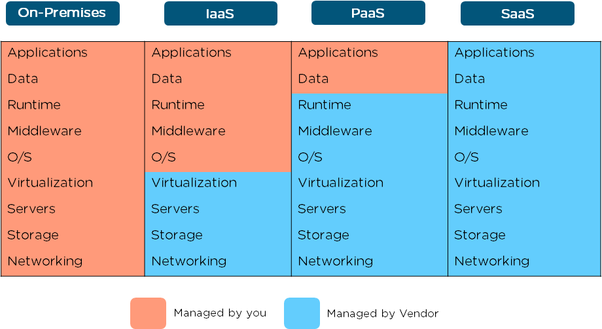
\includegraphics[width=10cm]{texfiles/images/cloud services comparison.png}
	\caption{Cloud Services Comparison \protect\cite{namitk2011}}
	\label{fig:my_label}
\end{figure}
Some random thing Some random thing Some random thing Some random thing Some random thing Some random thing Some random thing Some random thing Some random thing Some random thing Some random thing Some random thing Some random thing Some random thing Some random thing Some random thing Some random thing Some random thing Some random thing Some random thing Some random thing Some random thing Some random thing  
\section{Type of Anomalies}

Some random thing Some random thing Some random thing Some random thing Some random thing Some random thing Some random thing Some random thing Some random thing Some random thing Some random thing Some random thing Some random thing Some random thing Some random thing Some random thing Some random thing Some random thing Some random thing Some random thing Some random thing Some random thing Some random thing  


\begin{figure}[h]
	\centering
	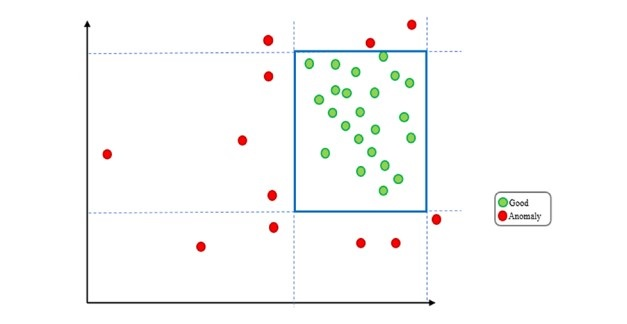
\includegraphics[width=10cm]{texfiles/images/image1.jpg}
	\caption{Simple Anomaly \protect\cite{Alla2019BeginningAD}}
	\label{fig:Figure 1}
\end{figure}
Some random thing Some random thing Some random thing Some random thing Some random thing Some random thing Some random thing Some random thing Some random thing Some random thing Some random thing Some random thing Some random thing Some random thing Some random thing Some random thing Some random thing Some random thing Some random thing Some random thing Some random thing Some random thing Some random thing  \cite{Sari2015}  

\subsection{Global anomaly}

Some random thing Some random thing Some random thing Some random thing Some random thing Some random thing Some random thing Some random thing Some random thing Some random thing Some random thing Some random thing Some random thing Some random thing Some random thing Some random thing Some random thing Some random thing Some random thing Some random thing Some random thing Some random thing Some random thing  
\begin{figure}
	\centering
	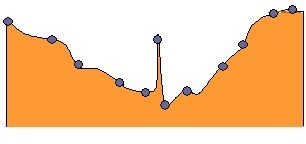
\includegraphics[width=10cm]{texfiles/images/global outlier.jpg}
	\caption{Global Anomaly \protect \cite{sayakpaul2019} }
	\label{fig:my_label}
\end{figure}

Some random thing Some random thing Some random thing Some random thing Some random thing Some random thing Some random thing Some random thing Some random thing Some random thing Some random thing Some random thing Some random thing Some random thing Some random thing Some random thing Some random thing Some random thing Some random thing Some random thing Some random thing Some random thing Some random thing  

\subsection{Contextual Anomaly}
Some random thing Some random thing Some random thing Some random thing Some random thing Some random thing Some random thing Some random thing Some random thing Some random thing Some random thing Some random thing Some random thing Some random thing Some random thing Some random thing Some random thing Some random thing Some random thing Some random thing Some random thing Some random thing Some random thing  
\begin{figure}[h]
	\centering
	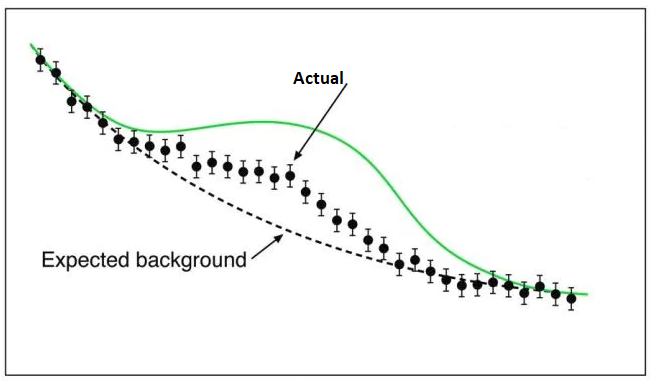
\includegraphics[width=10cm]{texfiles/images/contextual outlier.png}
	\caption{Contextual Anomaly Example \protect \cite{ABriefOv32:online}}
	\label{fig:my_label}
\end{figure}


Some random thing Some random thing Some random thing Some random thing Some random thing Some random thing Some random thing Some random thing Some random thing Some random thing Some random thing Some random thing Some random thing Some random thing Some random thing Some random thing Some random thing Some random thing Some random thing Some random thing Some random thing Some random thing Some random thing  
\subsection{Collective Anomaly}

Some random thing Some random thing Some random thing Some random thing Some random thing Some random thing Some random thing Some random thing Some random thing Some random thing Some random thing Some random thing Some random thing Some random thing Some random thing Some random thing Some random thing Some random thing Some random thing Some random thing Some random thing Some random thing Some random thing  
\begin{figure}[h]
	\centering
	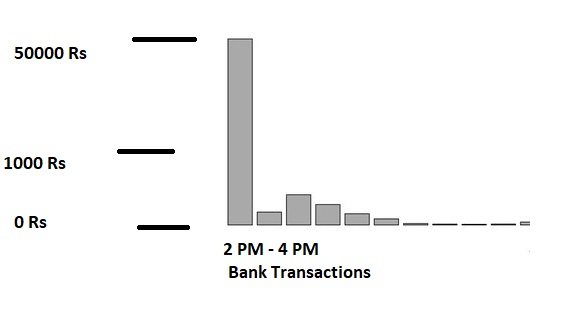
\includegraphics[width=10cm]{texfiles/images/collective anomaly.jpg}
	\caption{Collective Anomaly \protect\cite{Historic96:online}}
	\label{fig:my_label}
\end{figure}


Some random thing Some random thing Some random thing Some random thing Some random thing Some random thing Some random thing Some random thing Some random thing Some random thing Some random thing Some random thing Some random thing Some random thing Some random thing Some random thing Some random thing Some random thing Some random thing Some random thing Some random thing Some random thing Some random thing  

\begin{figure}[h]
	\centering
	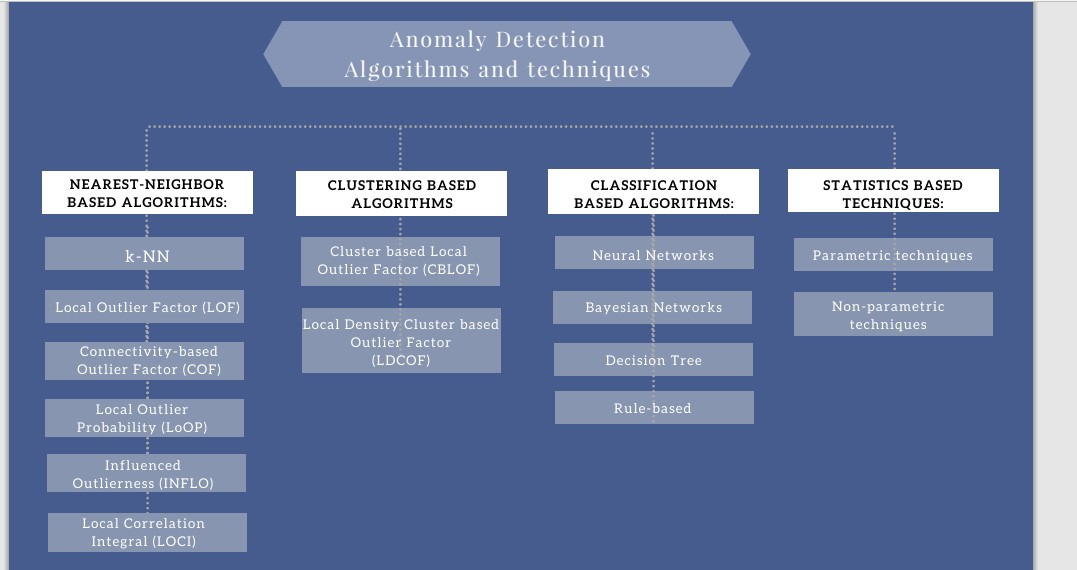
\includegraphics[width=10cm]{texfiles/images/anomaly-detection-algorithms.jpg}
	\caption{Anomaly Detection Algorithms \protect \cite{silviavalcheva} }
	\label{fig:my_label}
\end{figure}
Some random thing Some random thing Some random thing Some random thing Some random thing Some random thing Some random thing Some random thing Some random thing Some random thing Some random thing Some random thing Some random thing Some random thing Some random thing Some random thing Some random thing Some random thing Some random thing Some random thing Some random thing Some random thing Some random thing  

\subsection{Density-Based Anomaly Detection} 
Some random thing Some random thing Some random thing Some random thing Some random thing Some random thing Some random thing Some random thing Some random thing Some random thing Some random thing Some random thing Some random thing Some random thing Some random thing Some random thing Some random thing Some random thing Some random thing Some random thing Some random thing Some random thing Some random thing  
\subsection{Clustering-Based Anomaly Detection }

Some random thing Some random thing Some random thing Some random thing Some random thing Some random thing Some random thing Some random thing Some random thing Some random thing Some random thing Some random thing Some random thing Some random thing Some random thing Some random thing Some random thing Some random thing Some random thing Some random thing Some random thing Some random thing Some random thing  
%		 \begin{figure}[h]
%		     \centering
%		     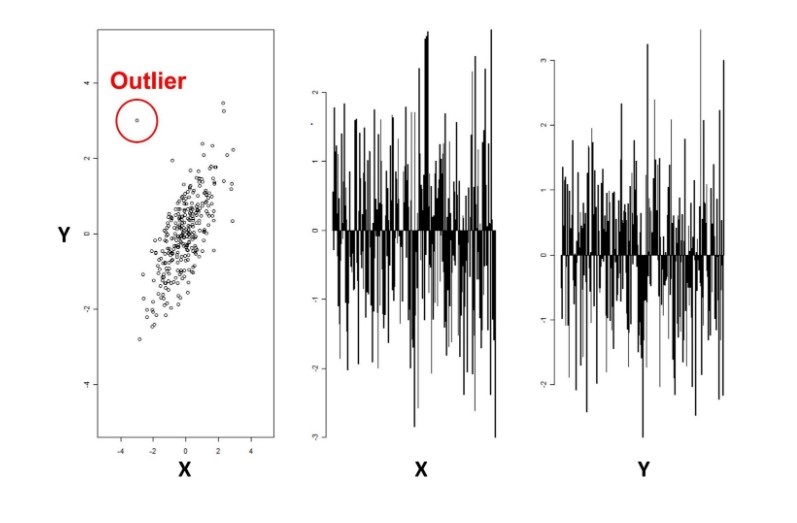
\includegraphics[width=10cm]{images/anomaly detection two variables.jpg}
%		     \caption{Collective Anomaly}
%		     \label{fig:my_label}
%		 \end{figure}
\subsection{Support Vector Machine-Based Anomaly Detection}


Some random thing Some random thing Some random thing Some random thing Some random thing Some random thing Some random thing Some random thing Some random thing Some random thing Some random thing Some random thing Some random thing Some random thing Some random thing Some random thing Some random thing Some random thing Some random thing Some random thing Some random thing Some random thing Some random thing  
\begin{figure}[ht]
	\centering
	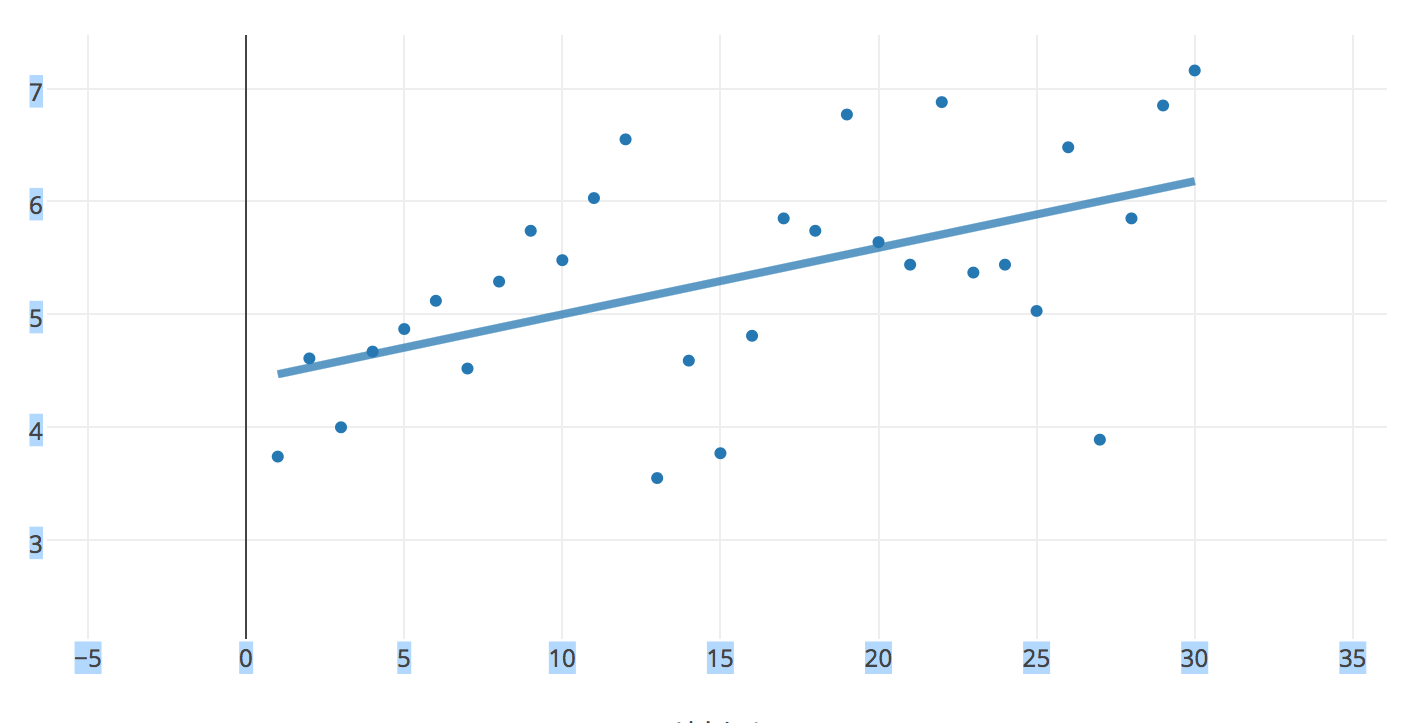
\includegraphics[width=10cm]{texfiles/images/2 variables.png}
	\caption{Anomaly detection using two variables \protect\cite{Generali53:online}}
	\label{fig:my_label}
\end{figure}
Some random thing Some random thing Some random thing Some random thing Some random thing Some random thing Some random thing Some random thing Some random thing Some random thing Some random thing Some random thing Some random thing Some random thing Some random thing Some random thing Some random thing Some random thing Some random thing Some random thing Some random thing Some random thing Some random thing  
\subsection{Anomaly detection algorithms categories}
Some random thing Some random thing Some random thing Some random thing Some random thing Some random thing Some random thing Some random thing Some random thing Some random thing Some random thing Some random thing Some random thing Some random thing Some random thing Some random thing Some random thing Some random thing Some random thing Some random thing Some random thing Some random thing Some random thing   \newline
\subsubsection{K-nearest neighbor: k-NN}

Some random thing Some random thing Some random thing Some random thing Some random thing Some random thing Some random thing Some random thing Some random thing Some random thing Some random thing Some random thing Some random thing Some random thing Some random thing Some random thing Some random thing Some random thing Some random thing Some random thing Some random thing Some random thing Some random thing  \newline

\subsubsection{Local Outlier Factor (LOF)} 

Some random thing Some random thing Some random thing Some random thing Some random thing Some random thing Some random thing Some random thing Some random thing Some random thing Some random thing Some random thing Some random thing Some random thing Some random thing Some random thing Some random thing Some random thing Some random thing Some random thing Some random thing Some random thing Some random thing  
\subsubsection{ K-means}

Some random thing Some random thing Some random thing Some random thing Some random thing Some random thing Some random thing Some random thing Some random thing Some random thing Some random thing Some random thing Some random thing Some random thing Some random thing Some random thing Some random thing Some random thing Some random thing Some random thing Some random thing Some random thing Some random thing  \newline
Some random thing Some random thing Some random thing Some random thing Some random thing Some random thing Some random thing Some random thing Some random thing Some random thing Some random thing Some random thing Some random thing Some random thing Some random thing Some random thing Some random thing Some random thing Some random thing Some random thing Some random thing Some random thing Some random thing  \newline
The user has to define the number of clusters in the early beginning.Some random thing Some random thing Some random thing Some random thing Some random thing Some random thing Some random thing Some random thing Some random thing Some random thing Some random thing Some random thing Some random thing Some random thing Some random thing Some random thing Some random thing Some random thing Some random thing Some random thing Some random thing Some random thing Some random thing  
\subsubsection{Support Vector Machine (SVM)} 

ASome random thing Some random thing Some random thing Some random thing Some random thing Some random thing Some random thing Some random thing Some random thing Some random thing Some random thing Some random thing Some random thing Some random thing Some random thing Some random thing Some random thing Some random thing Some random thing Some random thing Some random thing Some random thing Some random thing  
\subsubsection{Neural Networks Based Anomaly Detection}

Some random thing Some random thing Some random thing Some random thing Some random thing Some random thing Some random thing Some random thing Some random thing Some random thing Some random thing Some random thing Some random thing Some random thing Some random thing Some random thing Some random thing Some random thing Some random thing Some random thing Some random thing Some random thing Some random thing  \newpage

\begin{comment}

\textbf{Nearest-neighbor based algorithms:}
\begin{itemize}
\item k-NN
\item Local Outlier Factor (LOF)
\item Connectivity-based Outlier Factor (COF)
\item Local Outlier Probability (LoOP)
\item Influenced Outlierness (INFLO)
\item Local Correlation Integral (LOCI)
\end{itemize}
\textbf{Clustering based algorithms:}
\begin{itemize}
\item Cluster based Local Outlier Factor (CBLOF)
\item Local Density Cluster based Outlier Factor (LDCOF)
\end{itemize}
\textbf{Statistics based techniques:}
\begin{itemize}
\item Parametric techniques
\item Non-parametric techniques
\end{itemize}
\textbf{Classification based techniques:}
\begin{itemize}
\item Decision Tree
\item Neural Networks
\item Bayesian Networks
\item Rule-based.
\end{itemize}

\end{comment}

%anomaly detection algorithms conparison start here

\begin{comment}

\end{comment}

\begin{xltabular}{\textwidth}{@{} >{\raggedright\arraybackslash}X X X @{}} 
	\caption{Anomaly Detection Algorithms comparison\label{tab:algorithm_comp} \protect \cite{silviavalcheva} }\\
	
	\toprule      
	\kthead{Algorithm}   & \kthead{Pros}  & \kthead{Cons} \\ \midrule
	\begin{itemize}%
		%[label={}, wide = 0pt, leftmargin = *, nosep, itemsep = 0pt, before = \vspace*{\baselineskip}, after =\vspace*{\baselineskip} ]
		\item K Nearest Neighbour
		\item K-NN
	\end{itemize}   & \begin{enumerate}
		\item Very easy to understand 
		\item Good for creating models that include non standard data types such as
		text
	\end{enumerate}       & Large Storage requirements
	Computationally Expensive
	Sensitive to the choice of the similarity function for comparing instances             \\ \midrule
	Local Outlier Factor(LOF)  & Well-known and good algorithm
	for local anomaly detection
	& Only relies on its direct neighborhood .\newline Perform poorly on data sets with global anomalies. \\ \midrule
	K Means       & Low Complexity \newline Very easy to implement & Each cluster has pretty equal number of observations \newline Necessity of specifying K \newline Only work with numerical data \\ \midrule
	Support Vector Machine (SVM) & Find the best separation hyper-plane.Deal with very high dimensional data.\newline 
	Can learn very elaborate concepts.
	Work very well         & Require both positive and negative examples. Require lots of memory.\newline Some numerical stability problems.Need to select a good kernel function   \\ \midrule
	Neural networks based anomaly detection & Learns and does not need to be reprogrammed.\newline Can be implemented in any application  &    Needs training to operate \newline Requires high processing time for large neural networks \newline The architecture needs to be emulated          \\ \bottomrule
	
\end{xltabular}
Some random thing Some random thing Some random thing Some random thing Some random thing Some random thing Some random thing Some random thing Some random thing Some random thing Some random thing Some random thing Some random thing Some random thing Some random thing Some random thing Some random thing Some random thing Some random thing Some random thing Some random thing Some random thing Some random thing  
	\clearemptydoublepage
	\chapter{asasassas}
\label{chap:chapter3}
Some random thing Some random thing Some random thing Some random thing Some random thing Some random thing Some random thing Some random thing Some random thing Some random thing Some random thing Some random thing Some random thing Some random thing Some random thing Some random thing Some random thing Some random thing Some random thing Some random thing Some random thing Some random thing Some random thing  \\
\textbf{Keywords:} Some random thing Some random thing Some random thing Some random thing Some random thing Some random thing Some random thing Some random thing Some random thing Some random thing Some random thing Some random thing Some random thing Some random thing Some random thing Some random thing Some random thing Some random thing Some random thing Some random thing Some random thing Some random thing Some random thing  
%{abstract}

\section{kuttial}
Some random thing Some random thing Some random thing Some random thing Some random thing Some random thing Some random thing Some random thing Some random thing Some random thing Some random thing Some random thing Some random thing Some random thing Some random thing Some random thing Some random thing Some random thing Some random thing Some random thing Some random thing Some random thing Some random thing  \cite{density}
\section{lwoqsas}
Some random thing Some random thing Some random thing Some random thing Some random thing Some random thing Some random thing Some random thing Some random thing Some random thing Some random thing Some random thing Some random thing Some random thing Some random thing Some random thing Some random thing Some random thing Some random thing Some random thing Some random thing Some random thing Some random thing  \newline 
\textbf{Some} random thing Some random thing Some random thing Some random thing Some random thing Some random thing Some random thing Some random thing Some random thing Some random thing Some random thing Some random thing Some random thing Some random thing Some random thing Some random thing Some random thing Some random thing Some random thing Some random thing Some random thing Some random thing Some random thing  \cite{microsoft}
Some random thing Some random thing Some random thing Some random thing Some random thing Some random thing Some random thing Some random thing Some random thing Some random thing Some random thing Some random thing Some random thing Some random thing Some random thing Some random thing Some random thing Some random thing Some random thing Some random thing Some random thing Some random thing Some random thing  
\begin{figure}[h]
\begin{center}
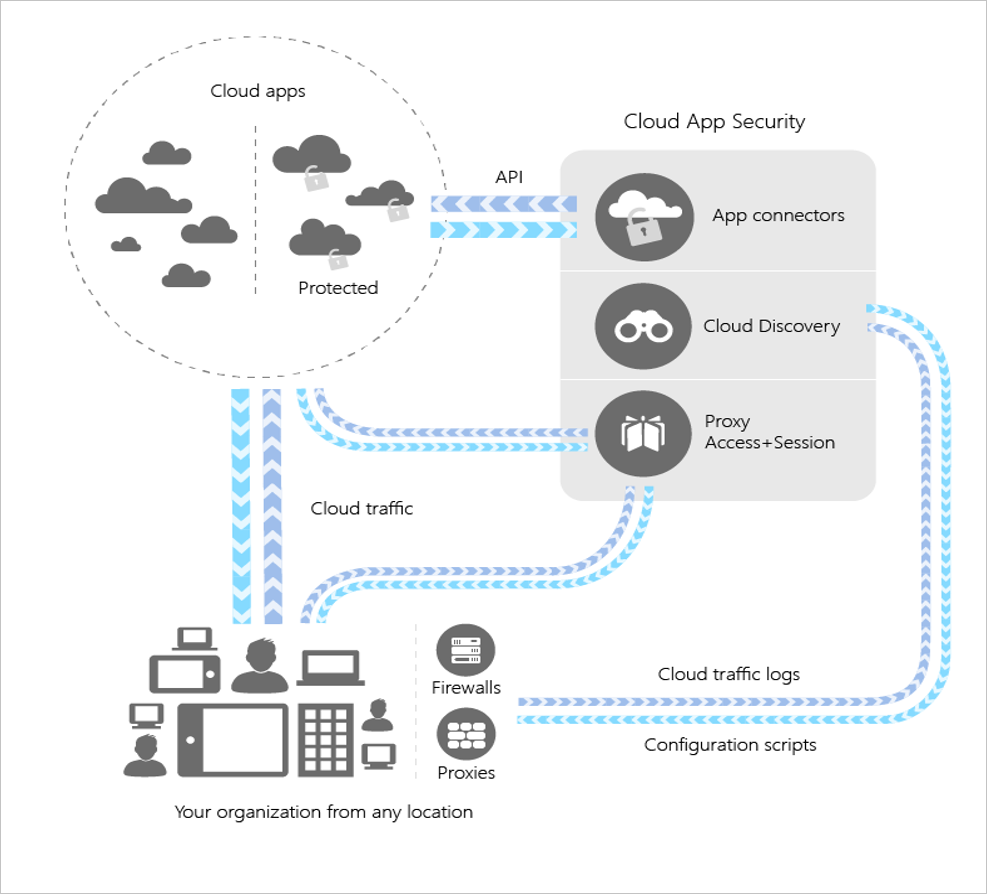
\includegraphics[width=10cm]{texfiles/images/proxy-architecture.png}
  \caption{Security architecture \protect\cite{WhatisCl88:online}}
  \label{fig:my_label}
\end{center}
\end{figure}
Some random thing Some random thing Some random thing Some random thing Some random thing Some random thing Some random thing Some random thing Some random thing Some random thing Some random thing Some random thing Some random thing Some random thing Some random thing Some random thing Some random thing Some random thing Some random thing Some random thing Some random thing Some random thing Some random thing  
\section{dsdsdsdsds}
Some random thing Some random thing Some random thing Some random thing Some random thing Some random thing Some random thing Some random thing Some random thing Some random thing Some random thing Some random thing Some random thing Some random thing Some random thing Some random thing Some random thing Some random thing Some random thing Some random thing Some random thing Some random thing Some random thing  \cite{microsf41} Some random thing Some random thing Some random thing Some random thing Some random thing Some random thing Some random thing Some random thing Some random thing Some random thing Some random thing Some random thing Some random thing Some random thing Some random thing Some random thing Some random thing Some random thing Some random thing Some random thing Some random thing Some random thing Some random thing   \\ Some random thing Some random thing Some random thing Some random thing Some random thing Some random thing Some random thing Some random thing Some random thing Some random thing Some random thing Some random thing Some random thing Some random thing Some random thing Some random thing Some random thing Some random thing Some random thing Some random thing Some random thing Some random thing Some random thing  \\
\begin{enumerate}
	\item Intc Threat Intelligence
	\item vioral Analytics
	\item uscdsdsion Analytics
\end{enumerate}
\subsection{Idsdssffs}  Some random thing Some random thing Some random thing Some random thing Some random thing Some random thing Some random thing Some random thing Some random thing Some random thing Some random thing Some random thing Some random thing Some random thing Some random thing Some random thing Some random thing Some random thing Some random thing Some random thing Some random thing Some random thing Some random thing  \newline 

\subsection{middddsds}  Some random thing Some random thing Some random thing Some random thing Some random thing Some random thing Some random thing Some random thing Some random thing Some random thing Some random thing Some random thing Some random thing Some random thing Some random thing Some random thing Some random thing Some random thing Some random thing Some random thing Some random thing Some random thing Some random thing  
Some random thing Some random thing Some random thing Some random thing Some random thing Some random thing Some random thing Some random thing Some random thing Some random thing Some random thing Some random thing Some random thing Some random thing Some random thing Some random thing Some random thing Some random thing Some random thing Some random thing Some random thing Some random thing Some random thing  .\newline 

\subsection{ddsdssfsfs}
Some random thing Some random thing Some random thing Some random thing Some random thing Some random thing Some random thing Some random thing Some random thing Some random thing Some random thing Some random thing Some random thing Some random thing Some random thing Some random thing Some random thing Some random thing Some random thing Some random thing Some random thing Some random thing Some random thing  \cite{fusion_analytics} Some random thing Some random thing Some random thing Some random thing Some random thing Some random thing Some random thing Some random thing Some random thing Some random thing Some random thing Some random thing Some random thing Some random thing Some random thing Some random thing Some random thing Some random thing Some random thing Some random thing Some random thing Some random thing Some random thing   \cite{mslinks2} Some random thing Some random thing Some random thing Some random thing Some random thing Some random thing Some random thing Some random thing Some random thing Some random thing Some random thing Some random thing Some random thing Some random thing Some random thing Some random thing Some random thing Some random thing Some random thing Some random thing Some random thing Some random thing Some random thing  
\section{sfsffssasas}
Some random thing Some random thing Some random thing Some random thing Some random thing Some random thing Some random thing Some random thing Some random thing Some random thing Some random thing Some random thing Some random thing Some random thing Some random thing Some random thing Some random thing Some random thing Some random thing Some random thing Some random thing Some random thing Some random thing  \cite{amazon2}.Some random thing Some random thing Some random thing Some random thing Some random thing Some random thing Some random thing Some random thing Some random thing Some random thing Some random thing Some random thing Some random thing Some random thing Some random thing Some random thing Some random thing Some random thing Some random thing Some random thing Some random thing Some random thing Some random thing  
 Events\cite{cloudwatch}, Some random thing Some random thing Some random thing Some random thing Some random thing Some random thing Some random thing Some random thing Some random thing Some random thing Some random thing Some random thing Some random thing Some random thing Some random thing Some random thing Some random thing Some random thing Some random thing Some random thing Some random thing Some random thing Some random thing  

\begin{figure}[h]
	\begin{center}
 	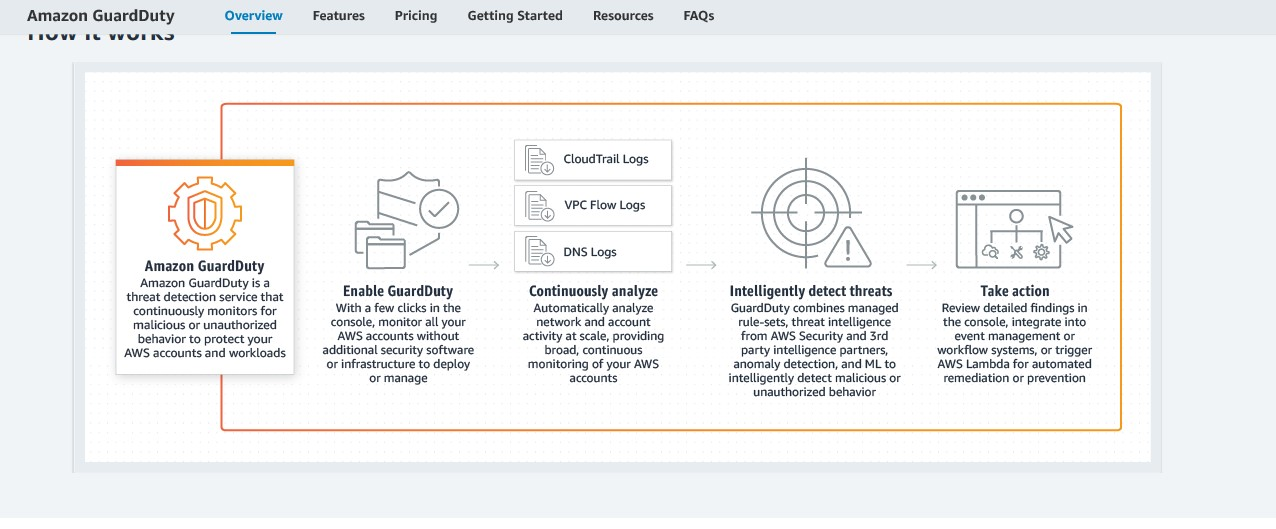
\includegraphics[width=15cm]{texfiles/images/gd.jpg}
\caption{Amazon Guard Duty \protect\cite{AmazonGu40:online}}\label{fig:my_label}
	\end{center}
\end{figure}

\section{dsdssdaaadad }
Some random thing Some random thing Some random thing Some random thing Some random thing Some random thing Some random thing Some random thing Some random thing Some random thing Some random thing Some random thing Some random thing Some random thing Some random thing Some random thing Some random thing Some random thing Some random thing Some random thing Some random thing Some random thing Some random thing  \cite{google31} which can
\begin{enumerate}
    \item Detect unusual firewall behaviors between snapshots.
    \item Alert users to any unusual behaviors and provide a comparison with expected behaviors.
    \item Provide potential remediation steps.
\end{enumerate}

Some random thing Some random thing Some random thing Some random thing Some random thing Some random thing Some random thing Some random thing Some random thing Some random thing Some random thing Some random thing Some random thing Some random thing Some random thing Some random thing Some random thing Some random thing Some random thing Some random thing Some random thing Some random thing Some random thing   \newline
\par
\begin{figure}[h]
\begin{center}
    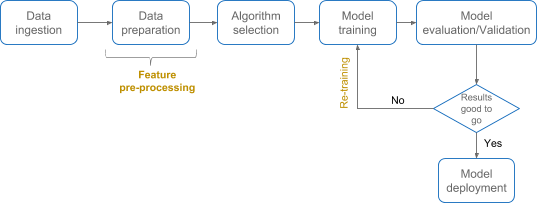
\includegraphics[width=14cm]{texfiles/images/security1.png}
\caption{ GCP Anomaly Detection \protect\cite{Identify70:online}}
\label{fig:gcp_ano}
\end{center}
   
\end{figure}
\section{addddadada}

Some random thing Some random thing Some random thing Some random thing Some random thing Some random thing Some random thing Some random thing Some random thing Some random thing Some random thing Some random thing Some random thing Some random thing Some random thing Some random thing Some random thing Some random thing Some random thing Some random thing Some random thing Some random thing Some random thing  
\begin{figure}[H]
\begin{center}
	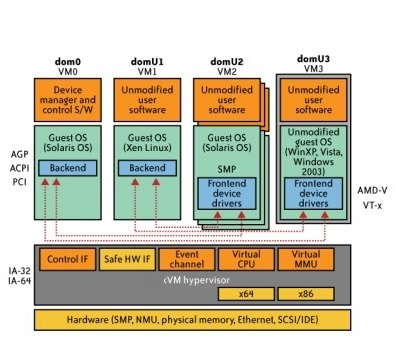
\includegraphics[width=15cm,height=60mm]{texfiles/images/hypervisor1.jpg}
  \caption{Hypervisor working \protect\cite{Virtuali40:online}}
  \label{fig:hypervisors} 
\end{center}
\end{figure}

\subsection{aadadd}

Some random thing Some random thing Some random thing Some random thing Some random thing Some random thing Some random thing Some random thing Some random thing Some random thing Some random thing Some random thing Some random thing Some random thing Some random thing Some random thing Some random thing Some random thing Some random thing Some random thing Some random thing Some random thing Some random thing   (See Table \ref{tab:technique-cat}).
\begin{table}[h!]
\begin{center}
\vspace{1ex}
\begin{tabular}{|c|c|} \hline
    {\bf Technique} & {\bf Category} \\\hline
    Supervised anomaly detection &   A\\
    \hline
    Semi Supervised Anomaly Detection & B \\ \hline
    Unsupervised anomaly detection & C\\
    \hline
\end{tabular}
\caption{\label{tab:technique-cat}Type of anomaly detection techniques.}
\end{center}
\end{table}

\section{Detectinsdd}
Some random thing Some random thing Some random thing Some random thing Some random thing Some random thing Some random thing Some random thing Some random thing Some random thing Some random thing Some random thing Some random thing Some random thing Some random thing Some random thing Some random thing Some random thing Some random thing Some random thing Some random thing Some random thing Some random thing  \cite{roch}, Some random thing Some random thing Some random thing Some random thing Some random thing Some random thing Some random thing Some random thing Some random thing Some random thing Some random thing Some random thing Some random thing Some random thing Some random thing Some random thing Some random thing Some random thing Some random thing Some random thing Some random thing Some random thing Some random thing  \cite{Sari2015}
Some random thing Some random thing Some random thing Some random thing Some random thing Some random thing Some random thing Some random thing Some random thing Some random thing Some random thing Some random thing Some random thing Some random thing Some random thing Some random thing Some random thing Some random thing Some random thing Some random thing Some random thing Some random thing Some random thing  
Some random thing Some random thing Some random thing Some random thing Some random thing Some random thing Some random thing Some random thing Some random thing Some random thing Some random thing Some random thing Some random thing Some random thing Some random thing Some random thing Some random thing Some random thing Some random thing Some random thing Some random thing Some random thing Some random thing  \cite{pannu} Some random thing Some random thing Some random thing Some random thing Some random thing Some random thing Some random thing Some random thing Some random thing Some random thing Some random thing Some random thing Some random thing Some random thing Some random thing Some random thing Some random thing Some random thing Some random thing Some random thing Some random thing Some random thing Some random thing  
Some random thing Some random thing Some random thing Some random thing Some random thing Some random thing Some random thing Some random thing Some random thing Some random thing Some random thing Some random thing Some random thing Some random thing Some random thing Some random thing Some random thing Some random thing Some random thing Some random thing Some random thing Some random thing Some random thing  \cite{dhanl}\newline
•	Ensemble techniques, using feature bagging,score normalization and different sources of diversity.\newline

Different methods perform differently  a lot on the data set and parameters, and methods it may have little systematic advantages over another when compared across many data sets and parameters.
Sample Anomaly Detection Problems. These examples show how anomaly detection might be used to find outliers in the training data or to score new, single-class data.
Algorithm for Anomaly Detection. Oracle Data Mining supports One-Class Support Vector Machine (SVM) Some random thing Some random thing Some random thing Some random thing Some random thing Some random thing Some random thing Some random thing Some random thing Some random thing Some random thing Some random thing Some random thing Some random thing Some random thing Some random thing Some random thing Some random thing Some random thing Some random thing Some random thing Some random thing Some random thing  \cite{CHEN20052617}Some random thing Some random thing Some random thing Some random thing Some random thing Some random thing Some random thing Some random thing Some random thing Some random thing Some random thing Some random thing Some random thing Some random thing Some random thing Some random thing Some random thing Some random thing Some random thing Some random thing Some random thing Some random thing Some random thing  \cite{capgemini1} Some random thing Some random thing Some random thing Some random thing Some random thing Some random thing Some random thing Some random thing Some random thing Some random thing Some random thing Some random thing Some random thing Some random thing Some random thing Some random thing Some random thing Some random thing Some random thing Some random thing Some random thing Some random thing Some random thing  

\section{asaddaddaaa}
Some random thing Some random thing Some random thing Some random thing Some random thing Some random thing Some random thing Some random thing Some random thing Some random thing Some random thing Some random thing Some random thing Some random thing Some random thing Some random thing Some random thing Some random thing Some random thing Some random thing Some random thing Some random thing Some random thing Some random thing Some random thing Some random thing Some random thing Some random thing Some random thing Some random thing Some random thing Some random thing Some random thing Some random thing Some random thing Some random thing Some random thing Some random thing Some random thing  \newline


	\clearemptydoublepage
	\chapter{PPPdsd}
\label{chap:chapter4}
Some random thing Some random thing Some random thing Some random thing Some random thing Some random thing Some random thing Some random thing Some random thing Some random thing Some random thing Some random thing Some random thing Some random thing Some random thing Some random thing Some random thing Some random thing Some random thing Some random thing Some random thing Some random thing Some random thing  
\begin{itemize}
    \item numpy
    \item pandas
    \item scikit-learn 
    \item matplotlib
\end{itemize}
Some random thing Some random thing Some random thing Some random thing Some random thing Some random thing Some random thing Some random thing Some random thing Some random thing Some random thing Some random thing Some random thing Some random thing Some random thing Some random thing Some random thing Some random thing Some random thing Some random thing Some random thing Some random thing Some random thing  \newline
\subsection{Data Description}
\textbf{Data Files:}Description of files used from data set\newline
kddcup.name A list of features.\newline
kddcup.data.gz The full data set (743 mb uncompressed)\newline
kddcup.data\textunderscore10percent.gz  A 10\% subset of original dataset.Was used to train the classifiers.\newline
kddcup.testdata.unlabeled\textunderscore10\_percent.gz
corrected.gz Test data with corrected labels.\newline
training\_attack\_types A list of intrusion types.\newline
\begin{figure}[H]
    \centering
    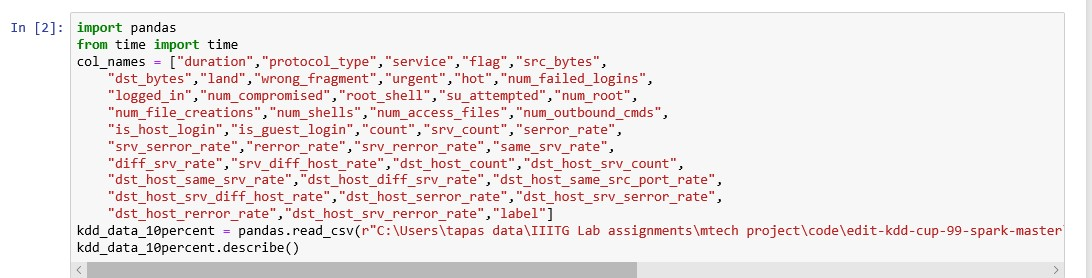
\includegraphics[width=15cm]{texfiles/images/code1.jpg}
    \caption{Initializing the dataset to feed in algorithm}
    \label{fig:code1}
\end{figure}
Some random thing Some random thing Some random thing Some random thing Some random thing Some random thing Some random thing Some random thing Some random thing Some random thing Some random thing Some random thing Some random thing Some random thing Some random thing Some random thing Some random thing Some random thing Some random thing Some random thing Some random thing Some random thing Some random thing  
\begin{figure}[H]
    \centering
    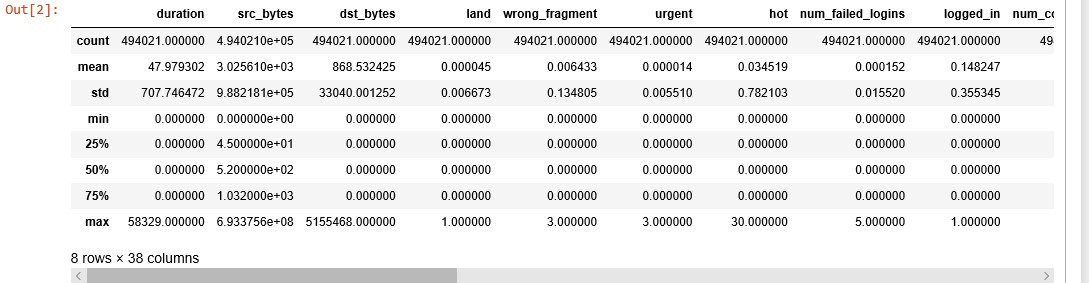
\includegraphics[width=15cm]{texfiles/images/code2.jpg}
    \caption{Output table generated after reading data}
    \label{fig:code2}
\end{figure}

Now we have our data loaded into a ``Pandas`` data frame. In order to get familiar with our data, let's have a look at how the labels are distributed. 
kdd\_data\_10percent['label'].value\_counts()
We get following attack types by reading the known attacks from the given dataset.
\begin{figure}[h]
    \centering
    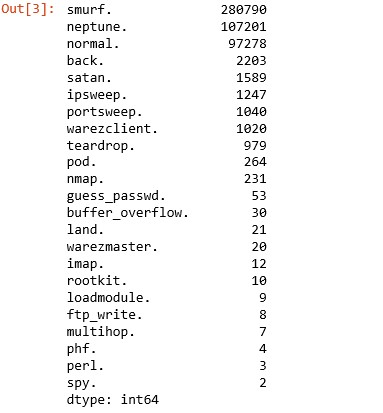
\includegraphics[height=7cm]{texfiles/images/code3.jpg}
    \caption{Attack types}
    \label{fig:code3}
\end{figure}
\subsection{Feature selection}

Some random thing Some random thing Some random thing Some random thing Some random thing Some random thing Some random thing Some random thing Some random thing Some random thing Some random thing Some random thing Some random thing Some random thing Some random thing Some random thing Some random thing Some random thing Some random thing Some random thing Some random thing Some random thing Some random thing  
\begin{comment}

Sklearn is a tool that helps dividing up the data into a test and a training set.
\begin{verbatim}
	from sklearn.model_selection import train_test_split
	
	features_train, features_test, labels_train, labels_test = train_test_split(
	features, labels, 
	test_size=0.20, random_state=42)
	
\end{verbatim}

Once the data is separated into test and training sets, we can begin to choose a classifier. 

\begin{verbatim}

	# import
from sklearn.neighbors import KNeighborsClassifier	

\end{verbatim}
KNearestneighbor can use any of the following 
algorithms ``auto``, ``ball\_tree``, ``kd\_tree``, ``brute``,the  default is ``auto``.
We can use any different classifier here other than RandomForestClassifier
sklearn is a toolkit which has various algorithms implemented and any of them can be choosen to 
implement a classifier depending upon what you want to do following shows implementation of RandomForestClassifier.

\begin{verbatim}
	# initialize
	clf = RandomForestClassifier()
	
	# train the classifier using the training data
	clf.fit(features_train, labels_train)
	
	# compute accuracy using test data
	acc_test = clf.score(features_test, labels_test)
	
	print ("Test Accuracy:", acc_test)
	
\end{verbatim}
A Some random thing Some random thing Some random thing Some random thing Some random thing Some random thing Some random thing Some random thing Some random thing Some random thing Some random thing Some random thing Some random thing Some random thing Some random thing Some random thing Some random thing Some random thing Some random thing Some random thing Some random thing Some random thing Some random thing  :
\begin{align}
	Precision &= \frac{True Positive}{True Positive+False Positive} \\
	Recall &= \frac{True Positive}{True Positive + False Negative} \\
	Accuracy(F1 score) &= 2 \times\frac{Precesion\times Recall}{Precision+Recall}
\end{align}

Some random thing Some random thing Some random thing Some random thing Some random thing Some random thing Some random thing Some random thing Some random thing Some random thing Some random thing Some random thing Some random thing Some random thing Some random thing Some random thing Some random thing Some random thing Some random thing Some random thing Some random thing Some random thing Some random thing  
\begin{verbatim}
from sklearn.metrics import recall_score, precision_score

precision = precision_score(labels_test, pred, average="weighted")
recall = recall_score(labels_test, pred, average="weighted")

print ("Precision:", precision) # 
print ("Recall:", recall) # 

\end{verbatim}

%\begin{figure}
%	\centering
%	\includegraphics{texfiles/images/}
%\end{figure}

Some random thing Some random thing Some random thing Some random thing Some random thing Some random thing Some random thing Some random thing Some random thing Some random thing Some random thing Some random thing Some random thing Some random thing Some random thing Some random thing Some random thing Some random thing Some random thing Some random thing Some random thing Some random thing Some random thing  
\begin{verbatim}
	from sklearn.svm import SVC
	clf = SVC
\end{verbatim}
Some random thing Some random thing Some random thing Some random thing Some random thing Some random thing Some random thing Some random thing Some random thing Some random thing Some random thing Some random thing Some random thing Some random thing Some random thing Some random thing Some random thing Some random thing Some random thing Some random thing Some random thing Some random thing Some random thing    
\begin{itemize}
	\item DOS: denial-of-service, e.g. syn flood;  
	\item R2L: unauthorized access from a remote machine, e.g. guessing password;  
	\item U2R:  unauthorized access to local superuser (root) privileges, e.g., various ``buffer overflow'' attacks;  
	\item probing: surveillance and other probing, e.g., port scanning.
\end{itemize}

 
 
  

	\clearemptydoublepage
	\chapter{Conclusion}
\label{chap:conclusion}
Some random thing Some random thing Some random thing Some random thing Some random thing Some random thing Some random thing Some random thing Some random thing Some random thing Some random thing Some random thing Some random thing Some random thing Some random thing Some random thing Some random thing Some random thing Some random thing Some random thing Some random thing Some random thing Some random thing  Some random thing Some random thing Some random thing Some random thing Some random thing Some random thing Some random thing Some random thing Some random thing Some random thing Some random thing Some random thing Some random thing Some random thing Some random thing Some random thing Some random thing Some random thing Some random thing Some random thing Some random thing Some random thing Some random thing  Some random thing Some random thing Some random thing Some random thing Some random thing Some random thing Some random thing Some random thing Some random thing Some random thing Some random thing Some random thing Some random thing Some random thing Some random thing Some random thing Some random thing Some random thing Some random thing Some random thing Some random thing Some random thing Some random thing  Some random thing Some random thing Some random thing Some random thing Some random thing Some random thing Some random thing Some random thing Some random thing Some random thing Some random thing Some random thing Some random thing Some random thing Some random thing Some random thing Some random thing Some random thing Some random thing Some random thing Some random thing Some random thing Some random thing  
	\clearemptydoublepage
	
	%\bibliographystyle{abbrv}
	%\clearemptydoublepage
	%\singlespace
	%\bibliography{biblio}
	
	
	%\cite{*}
	%\bibliographystyle{plain}
	%\bibliographystyle{alpha}
	\bibliographystyle{unsrt}
	\clearemptydoublepage
	\bibliography{biblio}
	%\addcontentsline{toc}{chapter}{References}
	
	%\input{texfiles/flat}
	%\clearemptydoublepage
	%\input{texfiles/nest}
	%\clearemptydoublepage
	%\input{texfiles/intent}
	%\clearemptydoublepage
	%\input{texfiles/lm}
	%\clearemptydoublepage
	%\input{texfiles/conclusions}
	%\clearemptydoublepage
	
	%\appendix
	
	%\bibliographystyle{abbrv}
	%\clearemptydoublepage
	%\singlespace
	%\bibliography{thesis}
	
	% \include{AppendixA}
	% \clearemptydoublepage
	% \include{AppendixB}
	% \clearemptydoublepage
	
	%\phantomsection \addcontentsline{toc}{chapter}{Index}
	%\renewcommand{\baselinestretch}{1} \small \normalsize
	\clearemptydoublepage
	
	\phantomsection \addcontentsline{toc}{chapter}{Author's Biography} %Optional
	\chapter*{}
 \begin{center}
 %\hrule height 0.5pt
 {\Huge \bfseries Author's Biography}
 \vspace{1cm}
 %\hrule height 0.5pt
 \end{center}
 
 \onehalfspace
 \noindent Tapas received his B. Tech \& MBA dual degree in Information Technology from ABV-IIITM, in 2009. He has been pursuing M. Tech at the Department of Computer Science and Engineering, IIIT Guwahati, since July 2018.
 %%%%%%%%%%%%%%%%%%%%%%%%%%%%%%%%%%%%%%%%%%%%%%%%5
 %\singlespace
 %\begin{center}
 %%\hrule height 0.5pt
 %\vspace{0.3cm}
 %{\bfseries {\large Publications made out of this thesis\\}}
 %(listed in reverse chronological order)
 %\vspace{0.3cm}
 %%\hrule height 0.5pt
 %\end{center}
 %
 %\begin{enumerate}
%\item Publication 1 in standard reference format
%\item Publication 2 in standard reference format

 	  
% \end{enumerate}
% some items in original tex files were commeneted those lines have double % in them.
\end{document}

%%%%%%%%%%%%%%%%%%
\if 0

\begin{figure}[tb]
	\centerline{
		\includegraphics[width=0.5\textwidth]{./figures/}
	}
	\caption{{\bf }}
	\label{fig:}
\end{figure}

\begin{figure*}[tb]
	\centerline{
		\subfloat[{\bf }]{\includegraphics[height=0.3\textwidth,width=3.5cm,angle=-90]{./figures/}}
		\hfil
		\subfloat[{\bf }]{\includegraphics[height=0.3\textwidth,width=3.5cm,angle=-90]{./figures/}}
		\hfil
		\subfloat[{\bf }]{\includegraphics[height=0.3\textwidth,width=3.5cm,angle=-90]{./figures/}}
	}
	\caption{{\bf }}
	\label{fig:}
\end{figure*}

\fi
%%%%%%%%%%%%%%%%%%
